\PassOptionsToPackage{unicode=true}{hyperref} % options for packages loaded elsewhere
\PassOptionsToPackage{hyphens}{url}
%
\documentclass[]{article}
\usepackage{lmodern}
\usepackage{amssymb,amsmath}
\usepackage{ifxetex,ifluatex}
\usepackage{fixltx2e} % provides \textsubscript
\ifnum 0\ifxetex 1\fi\ifluatex 1\fi=0 % if pdftex
  \usepackage[T1]{fontenc}
  \usepackage[utf8]{inputenc}
  \usepackage{textcomp} % provides euro and other symbols
\else % if luatex or xelatex
  \usepackage{unicode-math}
  \defaultfontfeatures{Ligatures=TeX,Scale=MatchLowercase}
\fi
% use upquote if available, for straight quotes in verbatim environments
\IfFileExists{upquote.sty}{\usepackage{upquote}}{}
% use microtype if available
\IfFileExists{microtype.sty}{%
\usepackage[]{microtype}
\UseMicrotypeSet[protrusion]{basicmath} % disable protrusion for tt fonts
}{}
\IfFileExists{parskip.sty}{%
\usepackage{parskip}
}{% else
\setlength{\parindent}{0pt}
\setlength{\parskip}{6pt plus 2pt minus 1pt}
}
\usepackage{hyperref}
\hypersetup{
            pdftitle={Strategy and Comms Coding Analyses (N=40)},
            pdfauthor={Matt Blanchard},
            pdfborder={0 0 0},
            breaklinks=true}
\urlstyle{same}  % don't use monospace font for urls
\usepackage[margin=1in]{geometry}
\usepackage{graphicx,grffile}
\makeatletter
\def\maxwidth{\ifdim\Gin@nat@width>\linewidth\linewidth\else\Gin@nat@width\fi}
\def\maxheight{\ifdim\Gin@nat@height>\textheight\textheight\else\Gin@nat@height\fi}
\makeatother
% Scale images if necessary, so that they will not overflow the page
% margins by default, and it is still possible to overwrite the defaults
% using explicit options in \includegraphics[width, height, ...]{}
\setkeys{Gin}{width=\maxwidth,height=\maxheight,keepaspectratio}
\setlength{\emergencystretch}{3em}  % prevent overfull lines
\providecommand{\tightlist}{%
  \setlength{\itemsep}{0pt}\setlength{\parskip}{0pt}}
\setcounter{secnumdepth}{5}
% Redefines (sub)paragraphs to behave more like sections
\ifx\paragraph\undefined\else
\let\oldparagraph\paragraph
\renewcommand{\paragraph}[1]{\oldparagraph{#1}\mbox{}}
\fi
\ifx\subparagraph\undefined\else
\let\oldsubparagraph\subparagraph
\renewcommand{\subparagraph}[1]{\oldsubparagraph{#1}\mbox{}}
\fi

% set default figure placement to htbp
\makeatletter
\def\fps@figure{htbp}
\makeatother

\usepackage{caption}
\captionsetup{labelsep = newline}
\captionsetup{justification = centering, singlelinecheck = false}
\usepackage{pdflscape}
\newcommand{\blandscape}{\begin{landscape}}
\newcommand{\elandscape}{\end{landscape}}
\usepackage{booktabs}
\usepackage{longtable}
\usepackage{array}
\usepackage{multirow}
\usepackage{wrapfig}
\usepackage{float}
\usepackage{colortbl}
\usepackage{pdflscape}
\usepackage{tabu}
\usepackage{threeparttable}
\usepackage{threeparttablex}
\usepackage[normalem]{ulem}
\usepackage{makecell}
\usepackage{xcolor}

\title{Strategy and Comms Coding Analyses (N=40)}
\author{Matt Blanchard}
\date{}

\begin{document}
\maketitle

\hypertarget{pca-on-strategy-variables}{%
\section{PCA on Strategy Variables}\label{pca-on-strategy-variables}}

\hypertarget{correlations-between-variables}{%
\subsection{Correlations between
variables}\label{correlations-between-variables}}

\begin{table}[H]

\caption{\label{tab:unnamed-chunk-2}Correlations between variables}
\centering
\fontsize{6}{8}\selectfont
\begin{tabular}[t]{llllll}
\toprule
  & 1 & 2 & 3 & 4 & 5\\
\midrule
1. MidIns\_Duration &  &  &  &  & \\
2. MidNon\_Duration & -.05 &  &  &  & \\
3. NormIns\_Duration & .32* & -.15 &  &  & \\
4. NormNon\_Duration & -.18 & -.09 & -.18 &  & \\
5. OppIns\_Duration & .39* & -.07 & .61** & -.18 & \\
\addlinespace
6. OppNon\_Duration & -.35* & .01 & -.56** & .12 & -.62**\\
\bottomrule
\end{tabular}
\end{table}

\hypertarget{kmo-and-bartletts-test-of-spherecity}{%
\subsection{KMO and Bartlett's Test of
Spherecity}\label{kmo-and-bartletts-test-of-spherecity}}

\begin{table}[H]

\caption{\label{tab:unnamed-chunk-4}KMO: Measure of sampling adequacy}
\centering
\fontsize{6}{8}\selectfont
\begin{tabular}[t]{r}
\toprule
KMO\\
\midrule
0.76\\
\bottomrule
\end{tabular}
\end{table}

\begin{table}[H]

\caption{\label{tab:unnamed-chunk-4}Bartletts test of spherecity}
\centering
\fontsize{6}{8}\selectfont
\begin{tabular}[t]{rlr}
\toprule
chisq & p.value & df\\
\midrule
48 & <.001 & 15\\
\bottomrule
\end{tabular}
\end{table}

\hypertarget{scree-plot}{%
\subsection{Scree plot}\label{scree-plot}}

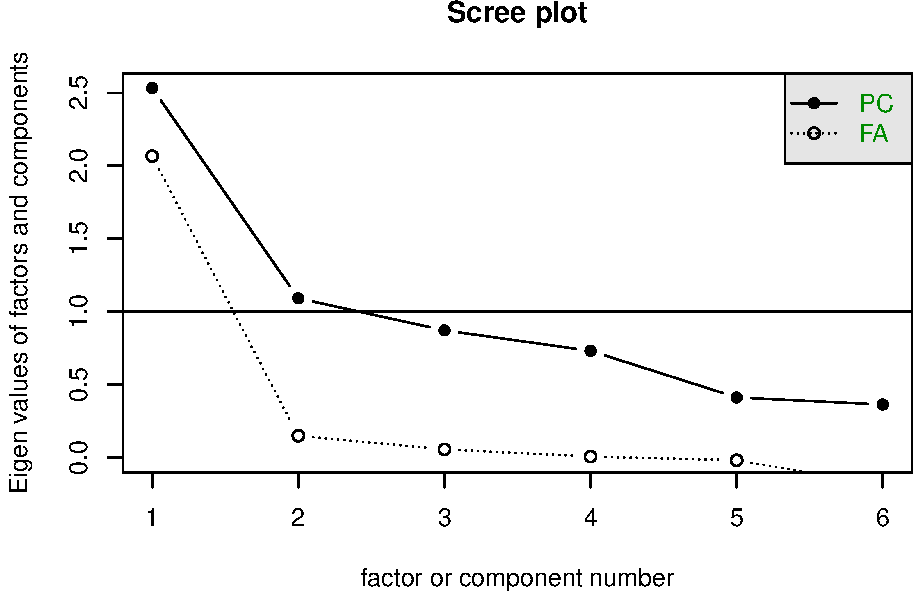
\includegraphics{strategy_comms_files/figure-latex/unnamed-chunk-5-1.pdf}

\hypertarget{pca-results}{%
\subsection{PCA results}\label{pca-results}}

\begin{table}[H]

\caption{\label{tab:unnamed-chunk-6}Variance accounted for by components}
\centering
\fontsize{6}{8}\selectfont
\begin{tabular}[t]{rrlll}
\toprule
component & eigen & prop\_var & cum\_var & rotation\_SS\_load\\
\midrule
1 & 2.53 & 0.42 & 0.42 & 2.53\\
2 & 1.09 & 0.18 & 0.6 & 1.09\\
3 & 0.87 &  &  & \\
4 & 0.73 &  &  & \\
5 & 0.41 &  &  & \\
\addlinespace
6 & 0.36 &  &  & \\
\bottomrule
\end{tabular}
\end{table}

\begin{table}[H]

\caption{\label{tab:unnamed-chunk-6}Pattern Matrix}
\centering
\fontsize{6}{8}\selectfont
\begin{tabular}[t]{lllr}
\toprule
var & PC1 & PC2 & h2\\
\midrule
OppIns\_Duration & 0.86 &  & 0.73\\
NormIns\_Duration & 0.83 &  & 0.68\\
MidIns\_Duration & 0.6 &  & 0.38\\
OppNon\_Duration & -0.81 &  & 0.65\\
MidNon\_Duration &  & 0.83 & 0.69\\
\addlinespace
NormNon\_Duration &  & -0.63 & 0.49\\
\bottomrule
\end{tabular}
\end{table}

PC1 = hesitant driving\\
PC2 = risky driving

\newpage

\hypertarget{pca-on-communication-variables}{%
\section{PCA on Communication
Variables}\label{pca-on-communication-variables}}

Due to the small sample size (N=40) we will conduct PCA separately for
positive and negative factors.

\hypertarget{reliability-for-each-communication-variable}{%
\subsection{Reliability for each communication
variable}\label{reliability-for-each-communication-variable}}

\begin{table}[H]

\caption{\label{tab:unnamed-chunk-7}Reliability}
\centering
\fontsize{6}{8}\selectfont
\begin{tabular}[t]{lr}
\toprule
Variable & alpha\\
\midrule
co\_info\_harm & 0.72\\
co\_info\_help & 0.86\\
co\_instruct\_harm & 0.61\\
co\_instruct\_help & 0.91\\
co\_question & 0.79\\
\addlinespace
co\_redundant & 0.72\\
drive\_frust & 0.91\\
drive\_informs & 0.82\\
drive\_question & 0.81\\
\bottomrule
\end{tabular}
\end{table}

\hypertarget{pca-for-positive-communication-variables-only}{%
\subsection{PCA for positive communication variables
only}\label{pca-for-positive-communication-variables-only}}

\hypertarget{correlations-between-variables-1}{%
\subsubsection{Correlations between
variables}\label{correlations-between-variables-1}}

\begin{table}[H]

\caption{\label{tab:unnamed-chunk-8}Correlations between variables}
\centering
\fontsize{6}{8}\selectfont
\begin{tabular}[t]{lllll}
\toprule
  & 1 & 2 & 3 & 4\\
\midrule
1. co\_info\_help\_overall &  &  &  & \\
2. co\_instruct\_help\_overall & .54** &  &  & \\
3. co\_question\_overall & .52** & .60** &  & \\
4. drive\_question\_overall & .65** & .56** & .40* & \\
5. drive\_informs\_overall & .67** & .54** & .69** & .48**\\
\bottomrule
\end{tabular}
\end{table}

\hypertarget{kmo-and-bartletts-test-of-spherecity-1}{%
\subsubsection{KMO and Bartlett's Test of
Spherecity}\label{kmo-and-bartletts-test-of-spherecity-1}}

\begin{table}[H]

\caption{\label{tab:unnamed-chunk-9}KMO: Measure of sampling adequacy}
\centering
\fontsize{6}{8}\selectfont
\begin{tabular}[t]{r}
\toprule
KMO\\
\midrule
0.79\\
\bottomrule
\end{tabular}
\end{table}

\begin{table}[H]

\caption{\label{tab:unnamed-chunk-9}Bartletts test of spherecity}
\centering
\fontsize{6}{8}\selectfont
\begin{tabular}[t]{rlr}
\toprule
chisq & p.value & df\\
\midrule
90 & <.001 & 10\\
\bottomrule
\end{tabular}
\end{table}

\hypertarget{scree-plot-1}{%
\subsubsection{Scree plot}\label{scree-plot-1}}

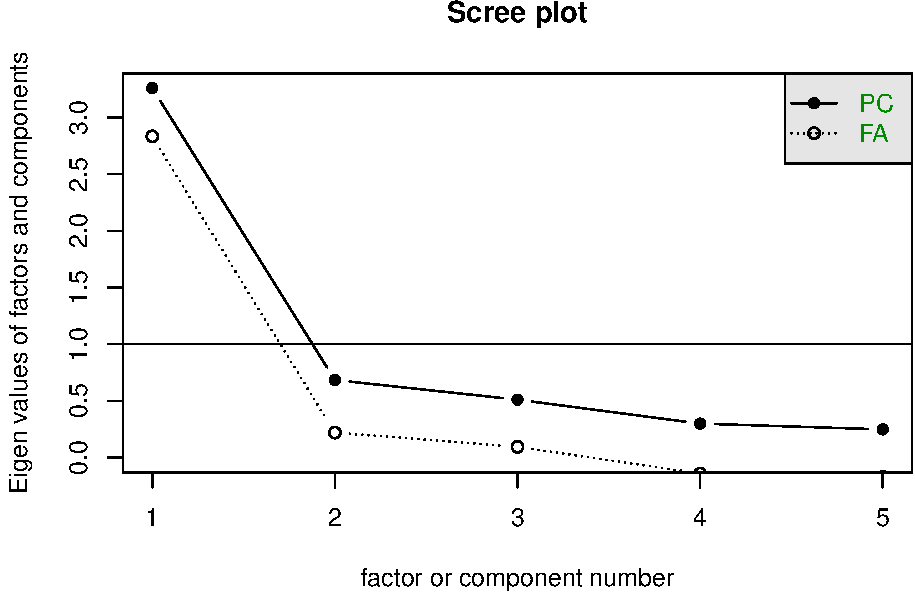
\includegraphics{strategy_comms_files/figure-latex/unnamed-chunk-10-1.pdf}

\hypertarget{pca-results-1}{%
\subsubsection{PCA results}\label{pca-results-1}}

\begin{table}[H]

\caption{\label{tab:unnamed-chunk-11}Variance accounted for by components}
\centering
\fontsize{6}{8}\selectfont
\begin{tabular}[t]{rrlll}
\toprule
component & eigen & prop\_var & cum\_var & rotation\_SS\_load\\
\midrule
1 & 3.26 & 0.65 & 0.65 & 3.26\\
2 & 0.68 &  &  & \\
3 & 0.51 &  &  & \\
4 & 0.30 &  &  & \\
5 & 0.25 &  &  & \\
\bottomrule
\end{tabular}
\end{table}

\begin{table}[H]

\caption{\label{tab:unnamed-chunk-11}Pattern Matrix}
\centering
\fontsize{6}{8}\selectfont
\begin{tabular}[t]{lrr}
\toprule
var & PC1 & h2\\
\midrule
co\_info\_help\_overall & 0.84 & 0.71\\
drive\_informs\_overall & 0.84 & 0.70\\
co\_instruct\_help\_overall & 0.80 & 0.64\\
co\_question\_overall & 0.80 & 0.64\\
drive\_question\_overall & 0.76 & 0.58\\
\bottomrule
\end{tabular}
\end{table}

PC1 = helpful exchange

\newpage

\hypertarget{pca-for-negative-communication-variables-only}{%
\subsection{PCA for negative communication variables
only}\label{pca-for-negative-communication-variables-only}}

\hypertarget{correlations-between-variables-2}{%
\subsubsection{Correlations between
variables}\label{correlations-between-variables-2}}

\begin{table}[H]

\caption{\label{tab:unnamed-chunk-12}Correlations between variables}
\centering
\fontsize{6}{8}\selectfont
\begin{tabular}[t]{llll}
\toprule
  & 1 & 2 & 3\\
\midrule
1. co\_info\_harm\_overall &  &  & \\
2. co\_instruct\_harm\_overall & .44** &  & \\
3. co\_redundant\_overall & .42** & .40** & \\
4. drive\_frust\_overall & .33* & .29 & .40*\\
\bottomrule
\end{tabular}
\end{table}

\hypertarget{kmo-and-bartletts-test-of-spherecity-2}{%
\subsubsection{KMO and Bartlett's Test of
Spherecity}\label{kmo-and-bartletts-test-of-spherecity-2}}

\begin{table}[H]

\caption{\label{tab:unnamed-chunk-13}KMO: Measure of sampling adequacy}
\centering
\fontsize{6}{8}\selectfont
\begin{tabular}[t]{r}
\toprule
KMO\\
\midrule
0.74\\
\bottomrule
\end{tabular}
\end{table}

\begin{table}[H]

\caption{\label{tab:unnamed-chunk-13}Bartletts test of spherecity}
\centering
\fontsize{6}{8}\selectfont
\begin{tabular}[t]{rlr}
\toprule
chisq & p.value & df\\
\midrule
26 & <.001 & 6\\
\bottomrule
\end{tabular}
\end{table}

\hypertarget{scree-plot-2}{%
\subsubsection{Scree plot}\label{scree-plot-2}}

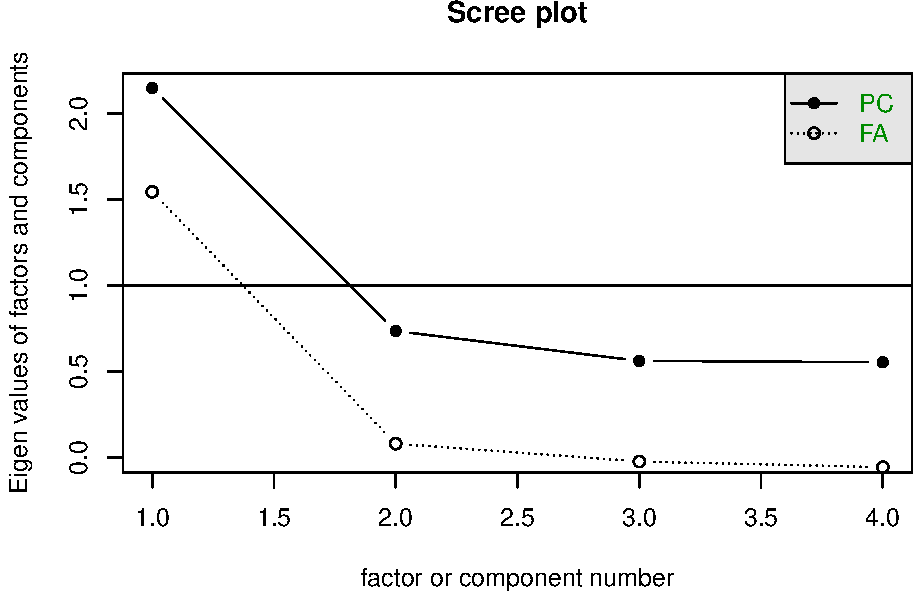
\includegraphics{strategy_comms_files/figure-latex/unnamed-chunk-14-1.pdf}

\hypertarget{pca-results-2}{%
\subsubsection{PCA results}\label{pca-results-2}}

\begin{table}[H]

\caption{\label{tab:unnamed-chunk-15}Variance accounted for by components}
\centering
\fontsize{6}{8}\selectfont
\begin{tabular}[t]{rrlll}
\toprule
component & eigen & prop\_var & cum\_var & rotation\_SS\_load\\
\midrule
1 & 2.15 & 0.54 & 0.54 & 2.15\\
2 & 0.74 &  &  & \\
3 & 0.56 &  &  & \\
4 & 0.55 &  &  & \\
\bottomrule
\end{tabular}
\end{table}

\begin{table}[H]

\caption{\label{tab:unnamed-chunk-15}Pattern Matrix}
\centering
\fontsize{6}{8}\selectfont
\begin{tabular}[t]{lrr}
\toprule
var & PC1 & h2\\
\midrule
co\_redundant\_overall & 0.77 & 0.59\\
co\_info\_harm\_overall & 0.76 & 0.58\\
co\_instruct\_harm\_overall & 0.73 & 0.53\\
drive\_frust\_overall & 0.67 & 0.45\\
\bottomrule
\end{tabular}
\end{table}

PC1 = harmful codriver

\newpage

\hypertarget{strategy-and-communication-factors-relationships}{%
\section{Strategy and Communication Factors
Relationships}\label{strategy-and-communication-factors-relationships}}

\hypertarget{correlations-with-simulation-derived-performance-metrics}{%
\subsection{Correlations with simulation derived performance
metrics}\label{correlations-with-simulation-derived-performance-metrics}}

\begin{table}[H]

\caption{\label{tab:unnamed-chunk-16}Correlations with performance metrics}
\centering
\fontsize{6}{8}\selectfont
\begin{tabular}[t]{lllllll}
\toprule
  & 1 & 2 & 3 & 4 & 5 & 6\\
\midrule
1. helpful\_exchange &  &  &  &  &  & \\
2. harmful\_codriver & .43** &  &  &  &  & \\
3. hesitant\_driving & .56** & .26 &  &  &  & \\
4. risky\_driving & -.07 & .00 & .13 &  &  & \\
5. collisions\_overall & .29 & .24 & -.01 & .19 &  & \\
\addlinespace
6. speed\_overall & -.46** & -.14 & -.12 & .34* & -.10 & \\
7. distance\_overall\_deviation & .36* & .52** & .34* & .20 & .32* & .04\\
\bottomrule
\end{tabular}
\end{table}

\newpage

\hypertarget{correlations-with-drivers-psychological-variables}{%
\subsection{Correlations with driver's psychological
variables}\label{correlations-with-drivers-psychological-variables}}

\begin{table}

\caption{\label{tab:unnamed-chunk-17}Correlations with driver's psychological variables}
\centering
\resizebox{\linewidth}{!}{
\begin{tabular}[t]{lllllllllllllllllllllllllll}
\toprule
  & 1 & 2 & 3 & 4 & 5 & 6 & 7 & 8 & 9 & 10 & 11 & 12 & 13 & 14 & 15 & 16 & 17 & 18 & 19 & 20 & 21 & 22 & 23 & 24 & 25 & 26\\
\midrule
1. helpful\_exchange &  &  &  &  &  &  &  &  &  &  &  &  &  &  &  &  &  &  &  &  &  &  &  &  &  & \\
2. harmful\_codriver & .43** &  &  &  &  &  &  &  &  &  &  &  &  &  &  &  &  &  &  &  &  &  &  &  &  & \\
3. hesitant\_driving & .56** & .26 &  &  &  &  &  &  &  &  &  &  &  &  &  &  &  &  &  &  &  &  &  &  &  & \\
4. risky\_driving & -.07 & .00 & .13 &  &  &  &  &  &  &  &  &  &  &  &  &  &  &  &  &  &  &  &  &  &  & \\
5. driving\_years & .05 & .01 & -.23 & -.13 &  &  &  &  &  &  &  &  &  &  &  &  &  &  &  &  &  &  &  &  &  & \\
\addlinespace
6. gaming\_time & .13 & .11 & .10 & .05 & -.16 &  &  &  &  &  &  &  &  &  &  &  &  &  &  &  &  &  &  &  &  & \\
7. congruent\_errors & -.22 & -.36* & -.18 & -.11 & -.17 & -.23 &  &  &  &  &  &  &  &  &  &  &  &  &  &  &  &  &  &  &  & \\
8. congruent\_time & .08 & -.04 & -.01 & -.11 & .34* & -.30 & -.11 &  &  &  &  &  &  &  &  &  &  &  &  &  &  &  &  &  &  & \\
9. incongruent\_errors & .13 & .03 & .02 & .15 & -.25 & .11 & .30 & -.49** &  &  &  &  &  &  &  &  &  &  &  &  &  &  &  &  &  & \\
10. incongruent\_time & .03 & .00 & .03 & -.11 & .29 & -.25 & -.23 & .88** & -.42** &  &  &  &  &  &  &  &  &  &  &  &  &  &  &  &  & \\
\addlinespace
11. inhibitory\_cost & -.06 & .06 & .08 & -.05 & .06 & -.05 & -.30 & .23 & -.08 & .67** &  &  &  &  &  &  &  &  &  &  &  &  &  &  &  & \\
12. repeat\_errors & .14 & .02 & -.10 & -.07 & -.21 & -.29 & .23 & -.19 & .58** & -.12 & .05 &  &  &  &  &  &  &  &  &  &  &  &  &  &  & \\
13. repeat\_time & .25 & .16 & .06 & -.19 & .18 & -.22 & -.16 & .60** & -.30 & .50** & .08 & -.13 &  &  &  &  &  &  &  &  &  &  &  &  &  & \\
14. switch\_errors & -.21 & -.01 & -.08 & .30 & -.22 & -.31 & .48** & -.12 & .43** & -.09 & .00 & .45** & -.31 &  &  &  &  &  &  &  &  &  &  &  &  & \\
15. switch\_time & .14 & .12 & -.03 & -.25 & .26 & -.30 & -.26 & .71** & -.44** & .61** & .13 & -.16 & .89** & -.34* &  &  &  &  &  &  &  &  &  &  &  & \\
\addlinespace
16. switch\_cost & -.14 & -.02 & -.18 & -.21 & .25 & -.26 & -.28 & .47** & -.40* & .42** & .13 & -.13 & .13 & -.18 & .56** &  &  &  &  &  &  &  &  &  &  & \\
17. wm\_accuracy & .05 & .23 & .14 & -.17 & .03 & .19 & -.10 & -.12 & .01 & -.12 & -.06 & -.13 & -.07 & .01 & -.02 & .08 &  &  &  &  &  &  &  &  &  & \\
18. resilience & .12 & .27 & -.09 & -.02 & .11 & -.02 & -.16 & -.08 & .19 & -.12 & -.13 & .28 & -.22 & -.06 & -.09 & .19 & .29 &  &  &  &  &  &  &  &  & \\
19. gf\_accuracy & .16 & .19 & .06 & -.15 & .20 & .40** & -.36* & -.23 & -.17 & -.10 & .16 & -.15 & -.08 & -.33* & -.03 & .07 & .42** & .14 &  &  &  &  &  &  &  & \\
20. confidence & .03 & .12 & .26 & .13 & -.28 & .44** & -.12 & -.62** & .12 & -.52** & -.09 & -.12 & -.26 & -.07 & -.37* & -.33* & .37* & .00 & .49** &  &  &  &  &  &  & \\
\addlinespace
21. bias & -.13 & -.07 & .20 & .28 & -.48** & .03 & .25 & -.37* & .29 & -.41** & -.25 & .02 & -.17 & .27 & -.33* & -.40** & -.05 & -.13 & -.52** & .49** &  &  &  &  &  & \\
22. discrimination & -.12 & -.26 & .00 & .04 & -.16 & .30 & -.19 & -.15 & .18 & -.13 & -.02 & -.06 & -.07 & -.03 & -.08 & -.03 & .29 & .01 & .25 & .05 & -.20 &  &  &  &  & \\
23. agreeableness & .56** & .26 & .32* & -.15 & .14 & .08 & .19 & .05 & .11 & .01 & -.06 & -.02 & .08 & .08 & -.03 & -.21 & .04 & .14 & .18 & .02 & -.16 & -.02 &  &  &  & \\
24. conscientiousness & .00 & .14 & .00 & -.11 & .10 & -.19 & .24 & .18 & -.06 & .07 & -.15 & -.21 & .13 & .05 & .09 & -.02 & .00 & .18 & -.13 & -.20 & -.06 & .08 & .38* &  &  & \\
25. extraversion & .18 & -.14 & .01 & .17 & .11 & -.30 & -.15 & .10 & -.02 & .03 & -.10 & .03 & .32* & -.09 & .30 & .06 & -.26 & -.01 & -.13 & -.21 & -.08 & .24 & -.07 & -.11 &  & \\
\addlinespace
26. intellect & -.29 & -.10 & -.11 & -.16 & .06 & .08 & .24 & -.20 & .04 & -.12 & .07 & -.25 & -.10 & .13 & -.15 & -.15 & .45** & -.03 & .12 & .19 & .06 & .10 & -.01 & -.16 & -.12 & \\
27. neuroticism & -.07 & -.02 & -.05 & -.12 & -.05 & -.23 & .29 & .07 & .09 & .15 & .20 & .22 & .21 & .21 & .05 & -.28 & .04 & -.26 & .03 & -.01 & -.04 & -.02 & -.07 & .07 & .04 & .23\\
\bottomrule
\end{tabular}}
\end{table}

\newpage

\hypertarget{correlations-with-codrivers-psychological-variables}{%
\subsection{Correlations with codriver's psychological
variables}\label{correlations-with-codrivers-psychological-variables}}

\begin{table}

\caption{\label{tab:unnamed-chunk-18}Correlations with codriver's psychological variables}
\centering
\resizebox{\linewidth}{!}{
\begin{tabular}[t]{lllllllllllllllllllllllllll}
\toprule
  & 1 & 2 & 3 & 4 & 5 & 6 & 7 & 8 & 9 & 10 & 11 & 12 & 13 & 14 & 15 & 16 & 17 & 18 & 19 & 20 & 21 & 22 & 23 & 24 & 25 & 26\\
\midrule
1. helpful\_exchange &  &  &  &  &  &  &  &  &  &  &  &  &  &  &  &  &  &  &  &  &  &  &  &  &  & \\
2. harmful\_codriver & .43** &  &  &  &  &  &  &  &  &  &  &  &  &  &  &  &  &  &  &  &  &  &  &  &  & \\
3. hesitant\_driving & .56** & .26 &  &  &  &  &  &  &  &  &  &  &  &  &  &  &  &  &  &  &  &  &  &  &  & \\
4. risky\_driving & -.07 & .00 & .13 &  &  &  &  &  &  &  &  &  &  &  &  &  &  &  &  &  &  &  &  &  &  & \\
5. driving\_years\_drone & .11 & -.12 & .14 & .21 &  &  &  &  &  &  &  &  &  &  &  &  &  &  &  &  &  &  &  &  &  & \\
\addlinespace
6. gaming\_time\_drone & -.16 & .02 & -.29 & -.03 & -.22 &  &  &  &  &  &  &  &  &  &  &  &  &  &  &  &  &  &  &  &  & \\
7. congruent\_errors\_drone & -.04 & -.25 & -.04 & -.01 & .01 & -.17 &  &  &  &  &  &  &  &  &  &  &  &  &  &  &  &  &  &  &  & \\
8. congruent\_time\_drone & -.19 & -.26 & -.17 & .00 & .36* & -.01 & -.10 &  &  &  &  &  &  &  &  &  &  &  &  &  &  &  &  &  &  & \\
9. incongruent\_errors\_drone & .12 & .13 & .07 & .15 & -.17 & .02 & .16 & -.59** &  &  &  &  &  &  &  &  &  &  &  &  &  &  &  &  &  & \\
10. incongruent\_time\_drone & -.19 & -.25 & -.22 & -.05 & .37* & .01 & -.23 & .82** & -.43** &  &  &  &  &  &  &  &  &  &  &  &  &  &  &  &  & \\
\addlinespace
11. inhibitory\_cost\_drone & -.03 & -.01 & -.10 & -.09 & .06 & .03 & -.23 & -.21 & .22 & .38* &  &  &  &  &  &  &  &  &  &  &  &  &  &  &  & \\
12. repeat\_errors\_drone & .15 & .27 & .13 & -.16 & -.09 & -.10 & .14 & -.11 & .23 & .01 & .20 &  &  &  &  &  &  &  &  &  &  &  &  &  &  & \\
13. repeat\_time\_drone & -.05 & .10 & -.27 & .10 & .17 & -.12 & -.17 & .53** & -.20 & .42** & -.13 & -.04 &  &  &  &  &  &  &  &  &  &  &  &  &  & \\
14. switch\_errors\_drone & .22 & .14 & .20 & -.15 & -.07 & .14 & .13 & -.03 & .21 & .12 & .25 & .74** & -.23 &  &  &  &  &  &  &  &  &  &  &  &  & \\
15. switch\_time\_drone & .03 & .00 & -.20 & .03 & .28 & -.16 & -.14 & .56** & -.30 & .44** & -.15 & -.13 & .88** & -.29 &  &  &  &  &  &  &  &  &  &  &  & \\
\addlinespace
16. switch\_cost\_drone & .14 & -.18 & .02 & -.11 & .32* & -.14 & -.02 & .31 & -.30 & .23 & -.10 & -.20 & .21 & -.22 & .64** &  &  &  &  &  &  &  &  &  &  & \\
17. wm\_accuracy\_drone & -.18 & .14 & -.07 & .06 & -.28 & .11 & -.11 & -.30 & .00 & -.32* & -.07 & -.14 & .04 & -.24 & -.05 & -.17 &  &  &  &  &  &  &  &  &  & \\
18. resilience\_drone & .28 & .16 & .10 & -.06 & -.13 & -.04 & -.09 & -.14 & .18 & -.22 & -.15 & -.16 & -.06 & .00 & .02 & .15 & .04 &  &  &  &  &  &  &  &  & \\
19. gf\_accuracy\_drone & -.17 & -.11 & .01 & .17 & -.03 & .12 & -.02 & -.22 & .13 & -.36* & -.27 & -.30 & -.29 & -.43** & -.21 & .04 & .22 & .01 &  &  &  &  &  &  &  & \\
20. confidence\_drone & .03 & .18 & .11 & .10 & -.28 & .07 & .18 & -.44** & .31 & -.52** & -.17 & -.13 & -.37* & -.17 & -.43** & -.29 & .37* & .18 & .46** &  &  &  &  &  &  & \\
\addlinespace
21. bias\_drone & .20 & .27 & .09 & -.09 & -.21 & -.07 & .17 & -.15 & .13 & -.07 & .13 & .21 & -.01 & .31 & -.15 & -.29 & .09 & .14 & -.65** & .38* &  &  &  &  &  & \\
22. discrimination\_drone & -.12 & -.20 & -.03 & .30 & .06 & .07 & -.03 & -.18 & .11 & -.12 & .08 & -.19 & -.26 & -.27 & -.18 & .06 & -.03 & .19 & .44** & .03 & -.43** &  &  &  &  & \\
23. agreeableness\_drone & .06 & .07 & .23 & -.02 & -.04 & .19 & .06 & .12 & .09 & .03 & -.15 & -.20 & -.08 & .03 & -.17 & -.22 & -.21 & .06 & -.11 & -.10 & .02 & -.14 &  &  &  & \\
24. conscientiousness\_drone & .08 & .03 & -.09 & .00 & .14 & -.23 & -.28 & -.08 & -.03 & -.14 & -.10 & -.26 & .22 & -.36* & .16 & -.03 & .17 & -.03 & -.08 & .09 & .16 & -.01 & -.15 &  &  & \\
25. extraversion\_drone & .19 & .04 & .00 & -.12 & .05 & .04 & .04 & .10 & .00 & -.02 & -.19 & -.10 & -.06 & -.01 & .03 & .15 & .06 & .34* & .00 & .22 & .18 & -.20 & .05 & -.02 &  & \\
\addlinespace
26. intellect\_drone & -.19 & .37* & -.14 & .16 & -.08 & .43** & -.22 & -.13 & .10 & -.14 & -.03 & .09 & .02 & -.13 & -.08 & -.19 & .37* & -.16 & .29 & .32* & -.03 & .22 & -.11 & .09 & .11 & \\
27. neuroticism\_drone & -.30 & -.05 & .01 & .14 & -.04 & -.07 & -.17 & .12 & .01 & .10 & -.02 & -.09 & .14 & -.27 & .09 & -.05 & .29 & -.31 & .37* & .14 & -.27 & .07 & .15 & .04 & -.10 & .15\\
\bottomrule
\end{tabular}}
\end{table}

\newpage

\hypertarget{correlations-with-drivers-nasa-tlx}{%
\subsection{Correlations with driver's
NASA-TLX}\label{correlations-with-drivers-nasa-tlx}}

\begin{table}[H]

\caption{\label{tab:unnamed-chunk-19}Correlations with driver's NASA-TLX}
\centering
\fontsize{6}{8}\selectfont
\begin{tabular}[t]{llllllllll}
\toprule
  & 1 & 2 & 3 & 4 & 5 & 6 & 7 & 8 & 9\\
\midrule
1. helpful\_exchange &  &  &  &  &  &  &  &  & \\
2. harmful\_codriver & .43** &  &  &  &  &  &  &  & \\
3. hesitant\_driving & .56** & .26 &  &  &  &  &  &  & \\
4. risky\_driving & -.07 & .00 & .13 &  &  &  &  &  & \\
5. effort & .30 & .22 & .19 & .00 &  &  &  &  & \\
\addlinespace
6. frustration & -.04 & .14 & -.06 & .08 & .02 &  &  &  & \\
7. mental\_demand & .25 & .31 & .17 & -.07 & .50** & .39* &  &  & \\
8. performance & .01 & -.14 & .28 & .06 & .08 & -.31 & .09 &  & \\
9. physical\_demand & -.12 & -.07 & -.07 & .10 & .20 & .31 & .10 & -.13 & \\
10. temporal\_demand & .19 & .20 & .09 & -.06 & .46** & .08 & .56** & .10 & .26\\
\bottomrule
\end{tabular}
\end{table}

\hypertarget{correlations-with-codrivers-nasa-tlx}{%
\subsection{Correlations with codriver's
NASA-TLX}\label{correlations-with-codrivers-nasa-tlx}}

\begin{table}[H]

\caption{\label{tab:unnamed-chunk-20}Correlations with codriver's NASA-TLX}
\centering
\fontsize{6}{8}\selectfont
\begin{tabular}[t]{llllllllll}
\toprule
  & 1 & 2 & 3 & 4 & 5 & 6 & 7 & 8 & 9\\
\midrule
1. helpful\_exchange &  &  &  &  &  &  &  &  & \\
2. harmful\_codriver & .43** &  &  &  &  &  &  &  & \\
3. hesitant\_driving & .56** & .26 &  &  &  &  &  &  & \\
4. risky\_driving & -.07 & .00 & .13 &  &  &  &  &  & \\
5. effort\_drone & .18 & .28 & .12 & .29 &  &  &  &  & \\
\addlinespace
6. frustration\_drone & -.13 & .00 & -.12 & .06 & .48** &  &  &  & \\
7. mental\_demand\_drone & .02 & .09 & -.19 & .18 & .49** & .64** &  &  & \\
8. performance\_drone & .08 & .18 & .15 & -.01 & -.08 & -.29 & -.16 &  & \\
9. physical\_demand\_drone & .02 & .18 & -.06 & .00 & .18 & .17 & .27 & .08 & \\
10. temporal\_demand\_drone & .11 & .13 & .06 & .22 & .56** & .55** & .71** & -.21 & .19\\
\bottomrule
\end{tabular}
\end{table}

\end{document}
